\documentclass{lug}
\usepackage{graphicx}
\usepackage{amsmath}
\usepackage{bm}
\usepackage{color}
\usepackage{pseudocode}
\usepackage{algorithmicx}
\usepackage{algpseudocode}
\usepackage{romannum}
\title{A Parallel Implementation of Random Forest}
\author{Lou Brand and Xun Li}
\institute{\textbf{Department of Computer Science\\Colorado School of Mines}}
\date{\today}

\begin{document}

\section{Background}
\frame{
    \frametitle{Random Forest}
    \begin{center}
        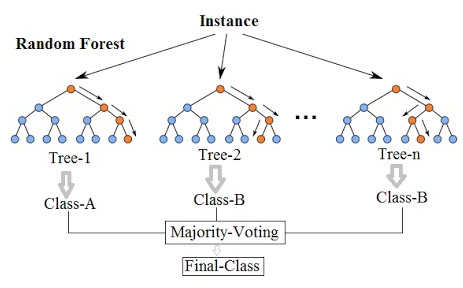
\includegraphics[scale=0.6]{images/random-forest-simplified.jpg}\\
        \textbf{Key:} Versatility
    \end{center}
}

\frame{
    \frametitle{gcForest}
    \begin{center}
        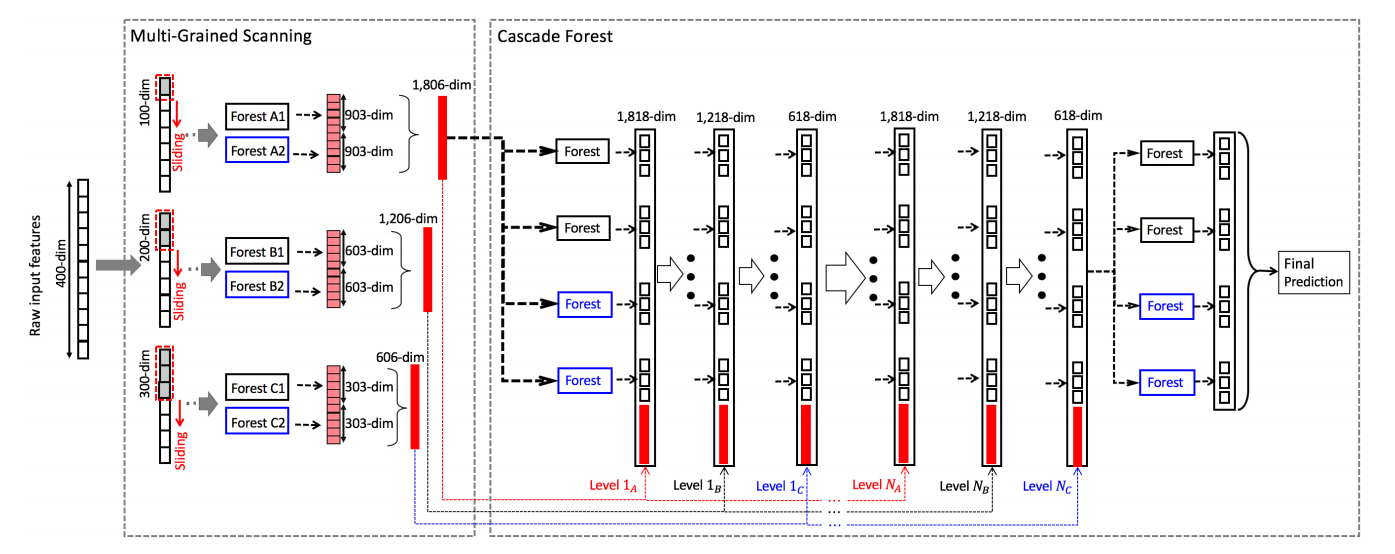
\includegraphics[scale=0.3]{images/gcForest.png}\\
        Find a quote from gcForest about ``easily'' parallelized. How did we misinterpret this initially? Where did this lead us? 
    \end{center}
}
\frame{
    \frametitle{Applications}
    \begin{center}
        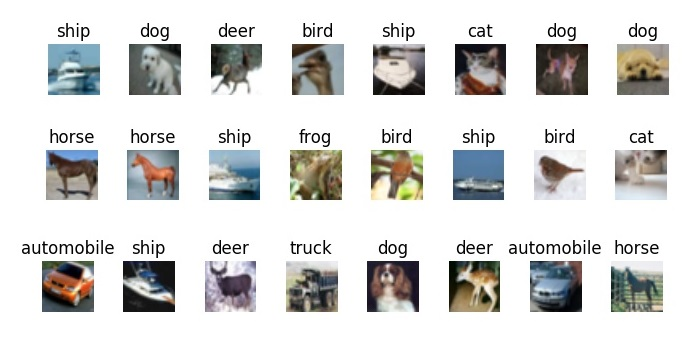
\includegraphics[scale=0.75]{images/cifar1.jpg}\\ 
        Face perception, image tagging, regression, classification, etc.
    \end{center}
}

\frame{
    \frametitle{An Insight into Node Splitting}
    \begin{itemize}[<+->]
        \item Focus on the elemental operation of the random forest algorithm
        \item Keep in mind.. tree algorithms are inherently difficult
            \begin{enumerate}
                \item Load balancing
                \item Dynamic irregular memory accesses
                \item As we get lower in the tree == many small kernels
            \end{enumerate}
    \end{itemize}
    \pause
    Can we use parallel programming on the CPU/GPU to give some insights into node splitting?
    Explicitly mention why we focus on node splitting and not the entire Random Forest algorithm.
}

\section{Approach}
\frame{
    \frametitle{Node Splitting}
    \begin{center}
        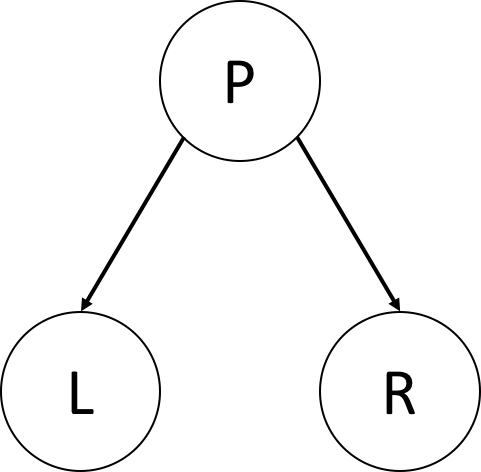
\includegraphics[scale=0.5]{images/node-split.png}\\
        \textbf{Goal}: Optimize splitting of the nodes using parallel programming techniques 
    \end{center}
}

\frame{
    \frametitle{Maximize Information Gain}
    \begin{center}
        Calculate Gini Index 
        $$ GI=1- \sum_{j=0}^{M}(\frac{C_j}{W})^2 $$
        $$ IG=GI_P-\frac{N_L}{N}GI_L-\frac{N_R}{N}GI_R $$
        Splitting value $= argmax(IG_{feature})$
    \end{center}
}

\frame{
    \frametitle{The Algorithm}
    \begin{pseudocode}{SplittingNodeNaive}{features} 
        1\quad \FOR k \GETS 0 \TO num(features)\\
        3\quad \quad ComputeHistogramForEachNode\\
        4\quad \quad ComputeGiniIndex\\
        5\quad \quad ComputeInformationGain\\
        6\quad split = argmax(InformationGain)\\
        7\quad \RETURN{split}
    \end{pseudocode}
}

\frame{
    \frametitle{Serial CPU Baseline}
    Talk about data. Put in timing data.
}

\section{GPU Implementation}

\frame{
    \frametitle{Ideas \Romannum{1}}
    
      \center \Large{Atomic block partitioning}
 %       \item Atomic interleaved partitioning
  %      \item Atomic privatization
   %     \item Coarse-grained embarrassing Parallelism 
    
}

\frame{
    \frametitle{GPU Implementation--atomic block} 
    
    a graph
    
}

\frame{
    \frametitle{Ideas \Romannum{2}}
    
      %\center Atomic block partitioning
      \center  \Large{Atomic interleaved partitioning}
  %      \item Atomic privatization
   %     \item Coarse-grained embarrassing Parallelism 
    
}


\frame{
    \frametitle{GPU Implementation--atomic interleaved} 
    
    a graph

    
    atomic throughput
}

\frame{
    \frametitle{Ideas \Romannum{3}}
    
      %\center Atomic block partitioning
      %\center  Atomic interleaved partitioning
        \center  \Large{privatization}
   %     \item Coarse-grained embarrassing Parallelism 
    
}


\frame{
    \frametitle{GPU Implementation--privatization} 
    
    a graph
    
}

\frame{
    \frametitle{Ideas \Romannum{4}}
    
      %\center Atomic block partitioning
      %\center  Atomic interleaved partitioning
        %\center  privatization
        \center \Large{Coarse-grained embarrassing Parallelism} 
    
}


\frame{
    \frametitle{GPU Implementation--Coarse-grain} 
    
    a graph
    
    utilization:
}
\section{Insights}

\frame{
    \frametitle{choice of backend}
    \begin{itemize}[<+->]
    	\item CPU serial: small dataset
        \item CPU parallel (OpenMP):
        \item GPU privation: 
        \item GPU coarse-grain:
    \end{itemize}
    \pause
     \begin{itemize}[<+->]
        \item GPU computation works well early on in the tree (when there are many instances to be bagged)
        \item Further down the tree the CPU implementation works best
    \end{itemize}
    
    Suggest random forest with clever backend choice in node splitting
}

\frame{
    \frametitle{Reuse \& Share in gcForest}
    \begin{itemize}
    	\item Algorithm improvements on redundancy
        \item The first node split can be precomputed and stored
        \item Task pool for node merge 
    \end{itemize}

}




\frame{
    \frametitle{Conclusions}
    \begin{itemize}
    	\item Four implementations of node splitting
        \item Understanding of performance bottleneck
        \item Insights into random forest optimizations 
    \end{itemize}

}


\frame{
    \begin{center}
        \Huge{Questions/Discussion}\\
    \end{center}
}

\nocite{*} % Include everything in the .bib file.
\bibliographystyle{plainnat}
\bibliography{random-forest-gpu}

% that's all, folks
\end{document}
